% id: 38-03
% book: 개념원리 중학 3-2 · 04 길이 구하기
% section: 개념원리 확인하기
% figure: crop:fig-38-03.png
% answer: $3$, $3$, $7$, $7$, $2\sqrt{19}$
% answer_source: 답지
% variant_level: 0 (원본 전사)
% 이 파일은 build.mjs 가 items.json 에서 만든다. 고칠 때는 items.json 을 고친다.
\smash{\raisebox{1.5mm}{\dmkichul{개념원리 중학 3-2 38쪽 03번}}}
\noindent\begin{minipage}[t]{0.58\linewidth}\vspace{0pt}\raggedright 다음은 오른쪽 그림과 같은 $\triangle\pt{ABC}$에서 $\seg{AB}=6$, $\seg{BC}=10$, $\angle\pt{B}=60^\circ$일 때, $\seg{AC}$의 길이를 구하는 과정이다. \blank\ 안에 알맞은 수를 써넣으시오.\end{minipage}\hfill\begin{minipage}[t]{0.4\linewidth}\vspace{0pt}\centering \setlength{\dmfigw}{102.0pt}\ifdim\dmfigw>\linewidth\setlength{\dmfigw}{\linewidth}\fi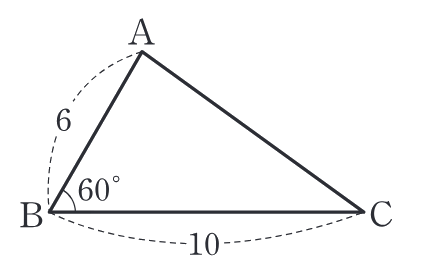
\includegraphics[width=\dmfigw]{figures/fig-38-03.png}\end{minipage}\par
\noindent \exprbox{\begin{minipage}{0.95\linewidth}\raggedright\setlength{\parskip}{1.5mm}오른쪽 그림과 같이 꼭짓점~$\pt{A}$에서 $\seg{BC}$에 내린 수선의 발을 $\pt{H}$라 하면 $\triangle\pt{ABH}$에서\par\hspace*{2em}$\seg{AH}=6\sin 60^\circ=3\sqrt{3}$, $\seg{BH}=6\cos 60^\circ=\blank$\par $\seg{CH}=\seg{BC}-\seg{BH}=10-\blank=\blank$이므로 $\triangle\pt{AHC}$에서\par\hspace*{2em}$\seg{AC}=\sqrt{(3\sqrt{3})^2+\blank^2}=\blank[2.5em]$\end{minipage}}
